%!TEX root = ../../main.tex


\begin{figure}[!htb]
\centering
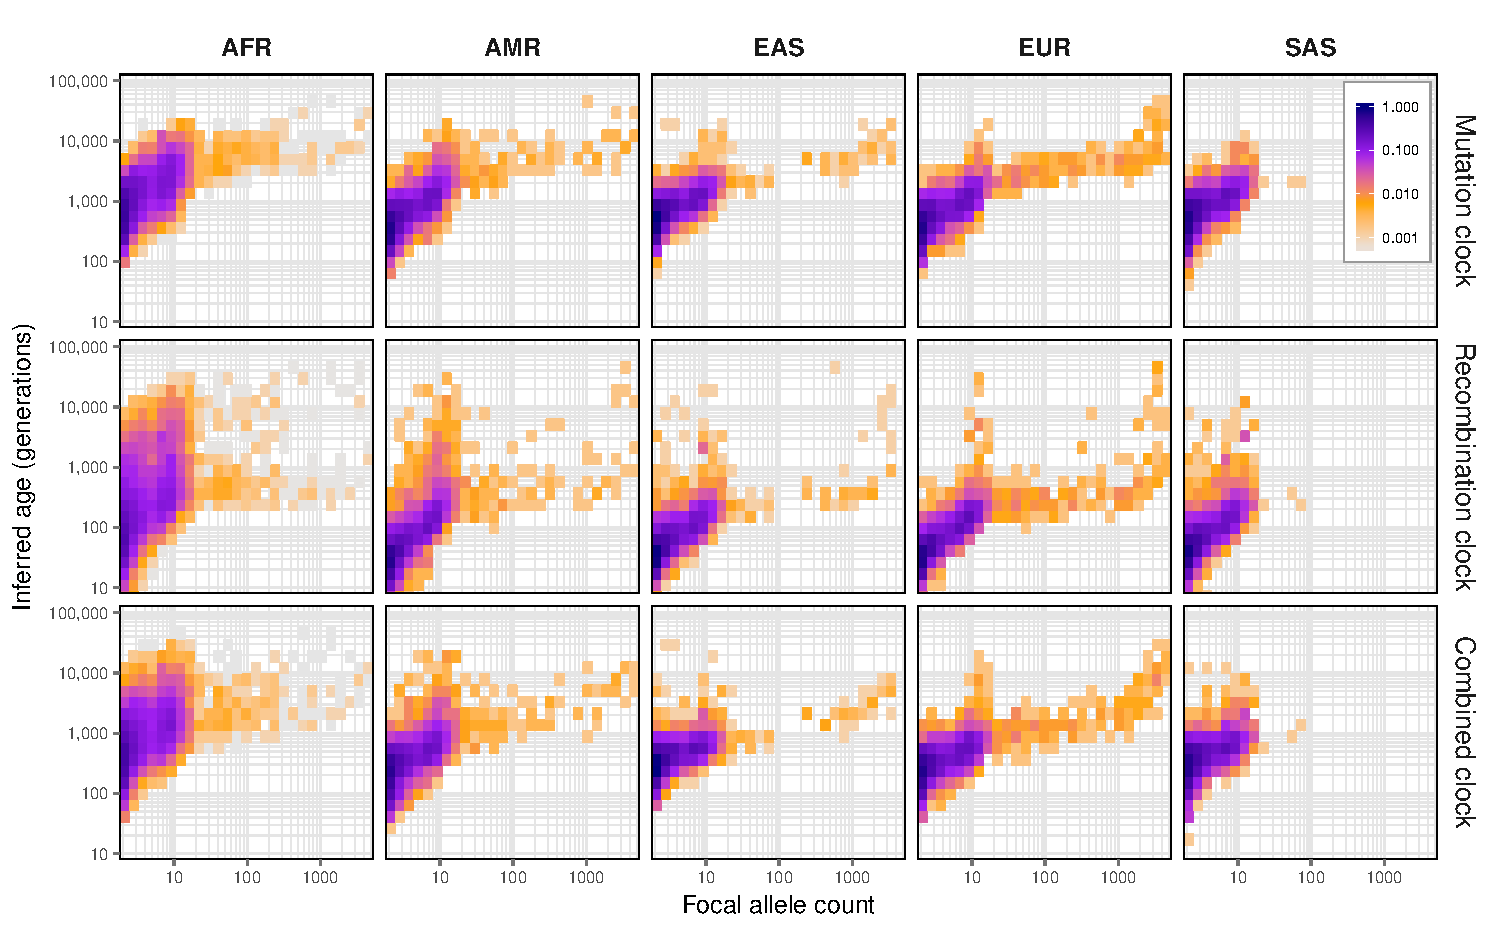
\includegraphics[width=\textwidth]{./img/ch5/1KG20_pop_age_hhmm}
\Caption{Allele age estimated by population in 1000 Genomes, chr.~20}%
{Age was estimated for alleles shared within the same population group contained in the \gls{1kg} sample, using the relaxed nearest neighbour approach to select discordant pairs.
Shared haplotype detection was performed using the haplotype-based \gls{hmm} and age was estimated under each of the three clock models (\ClockM, \ClockR, and \ClockC).
Colours indicate the maximised density of allele age by focal allele frequency.
Note that results are shown on log-log-scale.}%
{fig:1KG20_pop_age_hhmm}
\end{figure}
